\documentclass{ifaPoster}

\usepackage[utf8]{inputenc}
\usepackage[ngerman]{babel}
\usepackage{blindtext}
\usepackage{amsmath} % für multline
\usepackage{subfig} % für subfloat
\usepackage{todonotes}

\ifaAuthor{Meret Feldkemper}
\ifaTitle{Kollaborative Problemlösung in modularen Anlagen mittels persönlicher digitaler Assistenz}
\ifaSupervisorA{Dipl.-Ing. Sebastian Heinze}
%\ifaSupervisorB{Dipl.-Ing. Betreuer B}
%\ifaSupervisorC{Dipl.-Ing. Betreuer C}
\ifaProfessor{Prof. Dr.-Ing. habl. Leon Urbas}
\ifaDayOfSubmission{02.05.2019}
\ifaThesis{Diplomarbeit}
\ifaPhoto{DA_files/Passbild.jpg}
 
\begin{document}

\section{Motivation}
Durch Voranschreiten der Automatisierung in der Prozessführung sind Anlagenbediener vor allem in kritischen Situationen für Entscheidungen verantwortlich \cite{bainbridget_ironies_1983}. Der Mensch trifft seine Entscheidungen anhand von Beobachtungen und Erfahrungen. Im Zuge der entwickelten Modularisierungskonzept wird dies zunehmend schwieriger. Die Flexibilität der modularen Anlagen stellt die Anlagenbediener vor die Herausforderung, Probleme nicht mehr auf Grundlage von umfangreicher Erfahrung lösen zu können \cite{mueller_2018}. Assistenzsysteme bieten dem Anlagenbediener bei Erkennung von Problemen, deren Zusammenhängen und möglichen Lösungsansätzen Unterstützung. Dabei ist der Mensch mit einzubeziehen und seine Kompetenzen zu würdigen.

\section{Analyse}
Tritt ein Problem auf, muss der Nutzer darauf aufmerksam gemacht werden. Wichtig für das Assistenzsystem ist nicht nur die Einordnung, wodurch das Problem ausgelöst wurde, sondern auch wie zeitkritisch und wie komplex das Problem ist. Anhand dieser Merkmale sollte sich die Menge und Art der dargestellten Informationen orientieren. Aktuell erhält der Nutzer mit der Prozessführungsebene (PFE) nur eine Gesamtübersicht über den aktuellen Zustand der Anlage. Treten Meldungen auf, wird dem Nutzer nicht sichtbar gemacht, welcher Bereich betroffen ist und wie die Zusammenhänge sind.

Sollen Lösungen für ein entstandenes Problem gefunden werden, sind vor allem die Ziele eines produzierenden Unternehmens zu berücksichtigen. Diese reichen von der Verfügbarkeit von Mitarbeitern bis zum Aufwand Änderungen an der Anlage vorzunehmen.

\section{Konzept}
\begin{figure}[htbp]
\centering
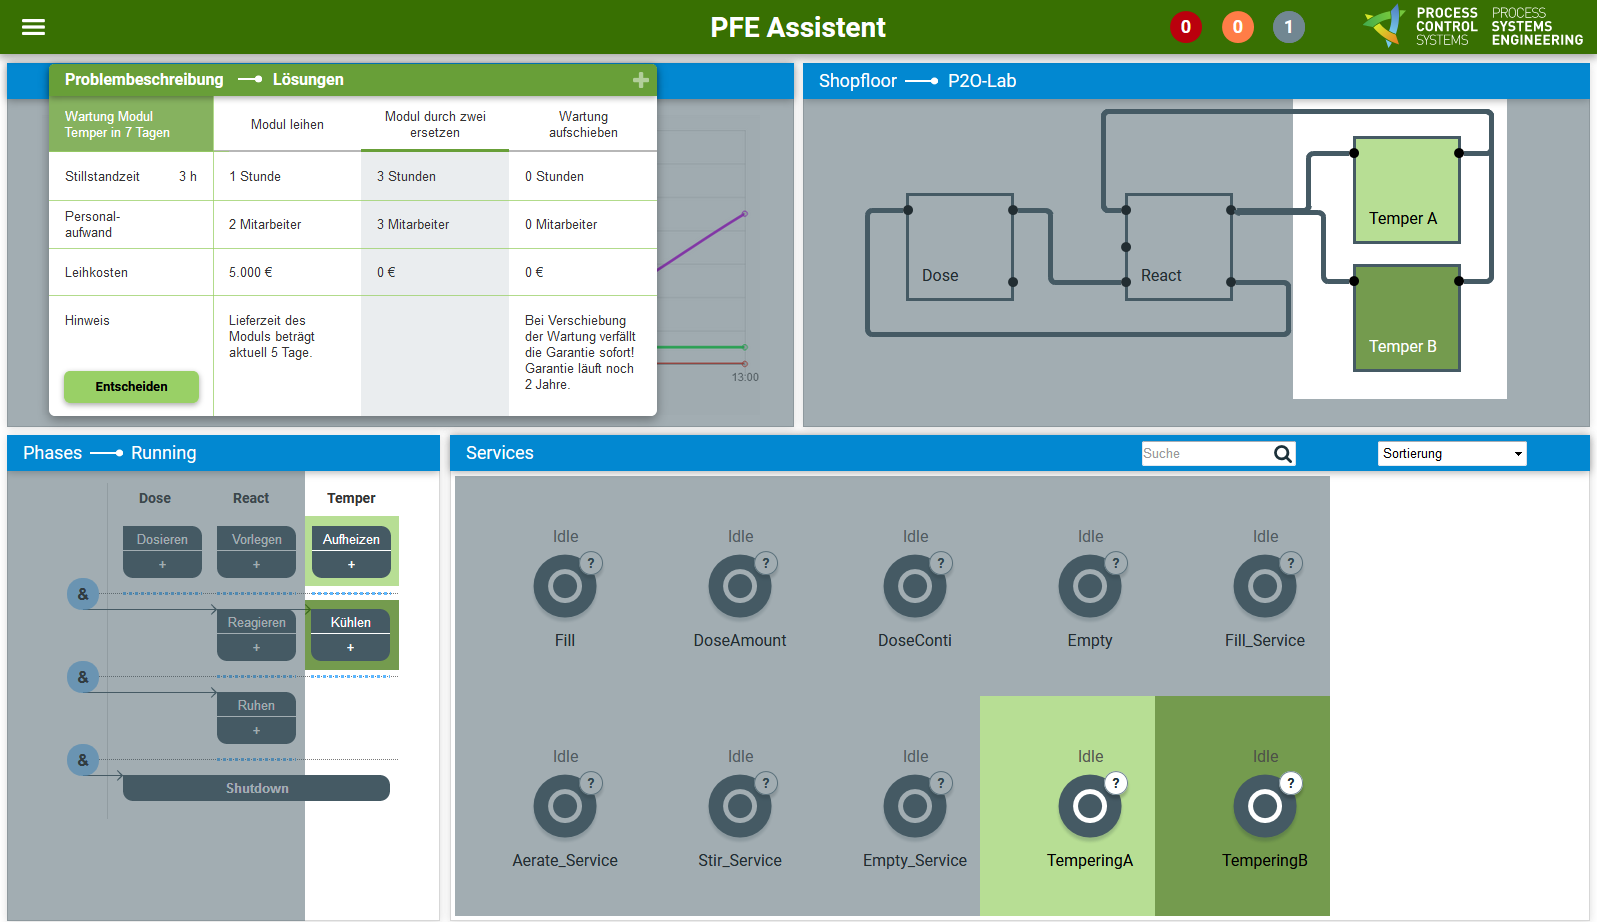
\includegraphics[scale=0.4]{DA_files/Prototyp-PFE-Loesung2.png}
\caption{Darstellung einer Lösung für ein Problem auf Grundlage der PFE}
\label{PFE-Loesungen}
\end{figure}

Das entwickelte User Interface baut auf einer bereits entwickelten PFE auf. Dies bietet den Vorteil, dass sich der Nutzer bei Anwendung des Assistenzsystem nicht an eine neue Benutzeroberfläche gewöhnen muss. Die Anpassung an den Problembereich wurde integriert, indem irrelevante Informationen versteckt werden. Der Nutzer kann durch die Anpassung der Ziele an die aktuellen Bedingungen im Unternehmen den Problemlöseprozess steuern. Anhand der eingegebenen Spezifikationen sucht das Assistenzsystem dann nach Lösungsmöglichkeiten, die dem Nutzer sowohl visuell als auch zahlenmäßig dargestellt werden (siehe Abbildung \ref{PFE-Loesungen}). Da ein Mensch 

 die der Nutzer begutachten kann, um eine Entscheidung zu treffen.


\section{Validierung}
Die Befragung einiger Experten zu dem vorgestellten Prototypen ergab ein insgesamt positive Bewertung. Sie schätzen insbesondere die gute Übersichtlichkeit und einfache Bedienung des Assistenzsystems. Besonders hervorgehoben wurde die Tatsache, dass die Assistenz bereits eine Vorauswahl an möglichen Zielen und Lösungen trifft. Dadurch wird der Nutzer nicht mit zu vielen Informationen überfordert. 


\section{Zusammenfassung und Ausblick}
Nutzer kann mit entsprechenden Informationen geeignet unterstützt werden. Offen bleibt, wie der Nutzer selber Probleme und Lösungen eingeben kann.


 {\tiny\renewcommand{\section}[2]{}%
 	 \begin{thebibliography}{8.5}
 	 \bibitem{bainbridget_ironies_1983}
 	 	Lisanne Bainbridget. {\glqq Ironies of Automation\grqq}. {In: \textit{Automatica}} 19.6 (1983), S. 775-779.
 	 \bibitem{mueller_2018}
 	 Romy Müller. {\glqq Cognitive challenges of changeability: adjustment
to system changes and transfer of knowledge in modular
chemical plants\grqq}. {In: \textit{Cognition, Technology and Work}} 21.1 (2018), S. 113-131.
	\end{thebibliography}}
	
\end{document}